\section{Studies}
\label{sec:studies}

The developed rapport system was tested using the Quick Numbers scenario (Figure~\ref{fig:quickNumbersScenario}) regarding likeability, intelligence and liveness using the Godspeed series~\cite{bartneck2009measurement, lehmann2015good}, and
	Proximity~\cite{aron1992inclusion}.

\begin{figure}[H]
	\centering
	\frame{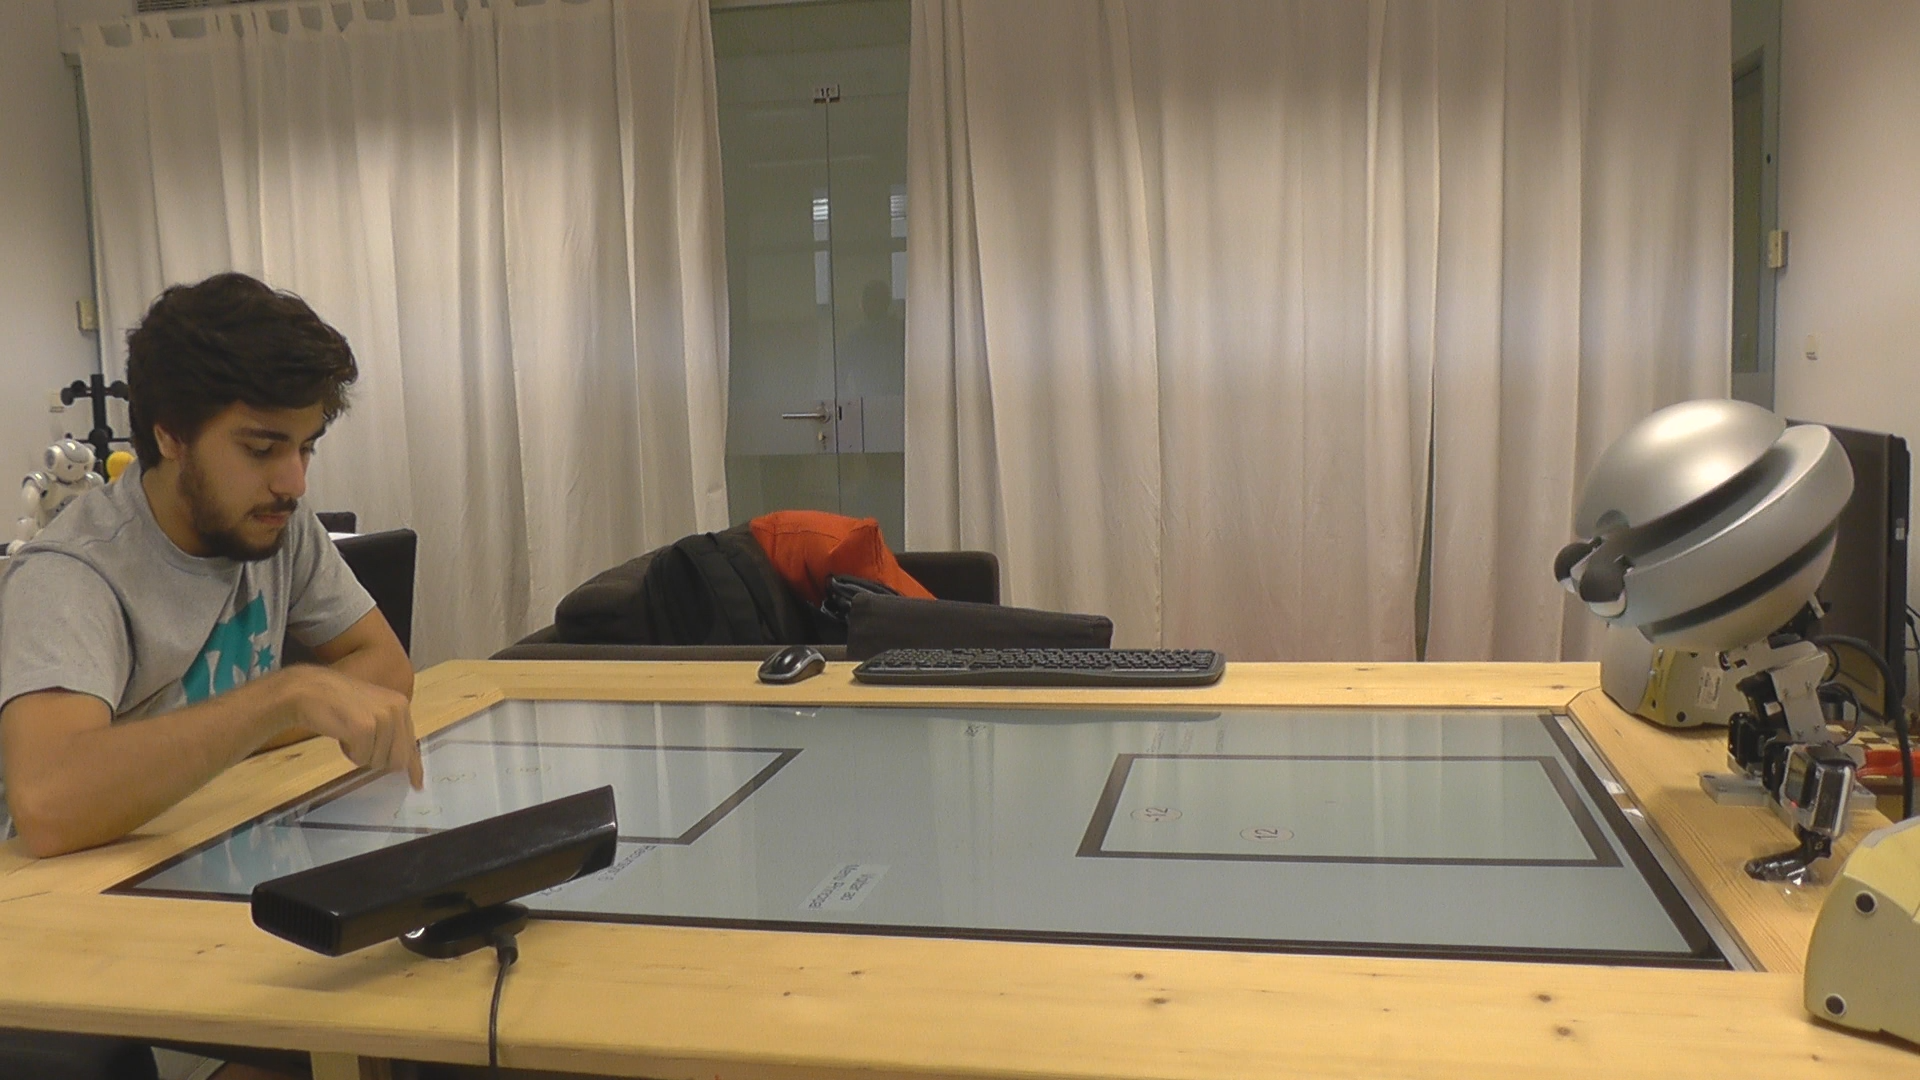
\includegraphics[width=0.35\textwidth]{ScenarioScreenShot.png}}
	\caption{An example of a participation in the Quick Numbers study (side view).}
	\label{fig:quickNumbersScenario}
\end{figure}

\subsection{Quick Numbers}

In the Quick Numbers scenario players are tasked with gaining as many resources as possible within the given time. At the beginning, each player starts with a fixed amount of resources that can be invested before each round. Depending on the amount invested and the player's performance, the returning investment will either be greater or lesser than the investment. The task is to tap the appearing numbers in sequential order starting with number one until the end of the round (Figure~\ref{fig:quickNumbers}). With each successful tap, the score increases, and with each incorrect number, the score decreases. In the end, the resources earned are the product between the amount invested and the round's score.

In this study, \ac{EMYS} accompanies the subject throughout the scenario, not as an opponent, but as another player that is also playing the game. The scenario stages go as follow:
\begin{itemize}
	\item \textbf{Introduction}: brief explanation of the rules, followed by the start the scenario;
	\item \textbf{Training Stage}: the participant plays an informal match alone to get accustomed to the game mechanics;
	\item \textbf{Gaming Session}: both players play a single round, at the same time;
	\item \textbf{Results Discussion}: the agent comments the each player scores;
	\item \textbf{Investment}: the participant is informed that he has to invest on the agent;
	\item \textbf{Ending}: \ac{EMYS} informs the value of the investment return and thanks to the subject for his participation.	
\end{itemize}

\begin{figure}[H]
	\centering
	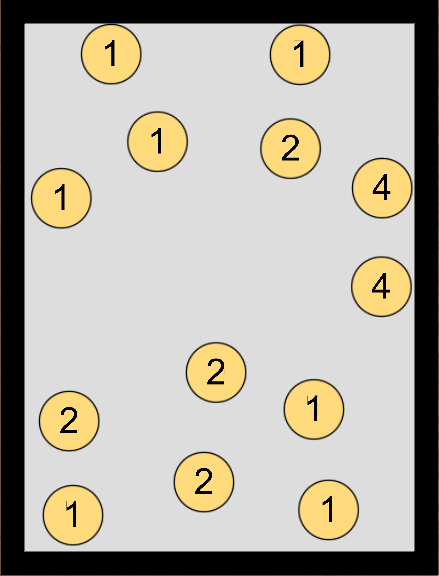
\includegraphics[width=0.2\textwidth]{FallingBoltsDiagram.png}
	\caption{Illustration of the Quick Numbers game developed in Unity.}
	\label{fig:quickNumbers}
\end{figure}

\subsection{Quick Numbers Plugins}

In addition to the plugins that implements the rapport model, we developed the following:
\begin{itemize}
	\item \textbf{Scenario \textit{Perceiver}}: monitors the scenario through \textit{Thalamus}, notifying the interested \textit{Effectors};
	\item \textbf{Utterances Manager}: proposes utterances according to the dyadic state of the interaction;
	\item \textbf{Rapport Strategies Manager}: enables/disables the rapport \textit{Effectors} throughout the scenario; 
\end{itemize}

The Utterances Manager \textit{Effector} implements the Positivity rapport \textit{Effector} and satisfies the ``Adhere to Social Norms'' goal of the rapport model by proposing utterances tailored to Quick Numbers (Table~\ref{fig:extended:utterances}). As the participant speaks Portuguese, different utterances are used depending on the subject's gender.

The Rapport Strategies Manager \textit{Effector} disables postural mimicry and mutual gaze rapport strategies during the Gaming Session and Investment stages, when \ac{EMYS} participates in Quick Numbers as a player and not as a spectator. In particular, it disables Facial Expression Mimicry \textit{Effector} in the investment phase because the participant's face is not visible on the video feed.

%This \textit{Effector} implements the positivity and the coordination component of the rapport model, proposing utterances according to the dyadic state of the interaction following the same structure as Table~\ref{fig:extended:utterances}. Given that \ac{EMYS} and the participant speak Portuguese, different utterances are used depending on the participant's gender. In addition to greeting and dismissing the participant, the rapport agent also: shares that it played sueca recently~\cite{correia2016trust}; motivates and praises the participant's performance; attempts to be humorous by saying ``I won't go anywhere... how could I? I am just a head...''.

\subsection{Results}
\label{sec:results}

A group of 40 participants from different universities campus participated in this study. The participants were equally selected and randomly distributed between the control condition (C) and the rapport condition (R), making two independent groups. Condition C has a mean age of 23.5±1, equal distribution of genders, and over 55\% of the participants already interacted with \ac{EMYS}. Condition R has a mean age of 25.65±3.945, 60\% male and only 25\% of the sample played with \ac{EMYS} in the past.

The study follows a between-subjects design, using significance level of 5\% for every statistical analysis.

\subsection*{\textbf{\textit{Are the rapport strategies effective in making agents more likeable?}}}

From the questionnaires, we compared the likability statistics between condition C (Figure~\ref{fig:likability_baseline}) and R (Figure~\ref{fig:likability_rapport}). As the distributions do not follow a normal distribution on both conditions ($sig_C=0.001$ and $sig_R=0$), we compare them with the \textit{Mann–Whitney U} statistical test. As the histogram's shapes are dissimilar ($sig=0.201$), we can only compare the mean scores: 5.0±0.649 and 5.3±0.865, on conditions C and R, respectively.

\begin{figure}[ht]
	\centering
	\begin{minipage}[b]{.2\textwidth}
		\centering
		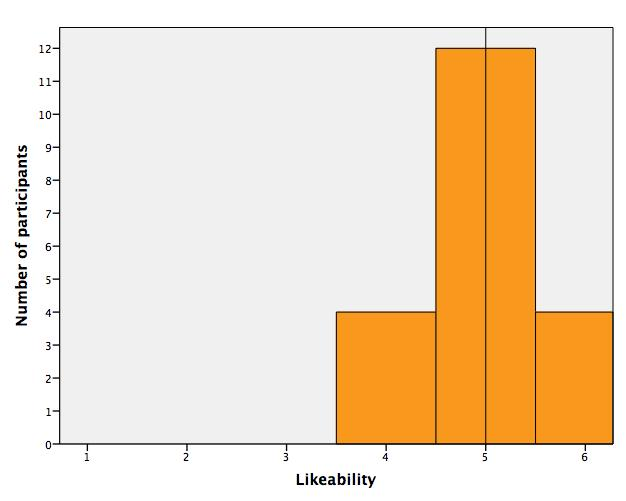
\includegraphics[width=\textwidth]{LikabilityBaseline.jpeg}
		\caption{Likeability histogram in the control condition.}
		\label{fig:likability_baseline}
	\end{minipage}
	\hspace{2mm}
	\begin{minipage}[b]{.2\textwidth}
		\centering
		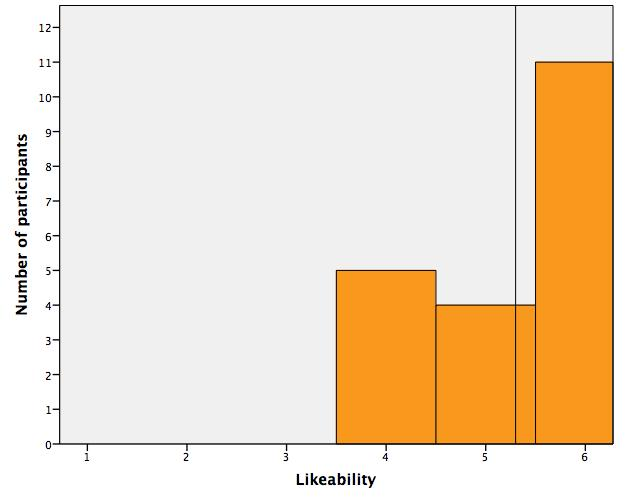
\includegraphics[width=\textwidth]{LikabilityRapport.jpeg}
		\caption{Likeability histogram in the rapport condition.}
		\label{fig:likability_rapport}
	\end{minipage}
\end{figure}



\textbf{Answer}: Despite the greater man average on the rapport condition, there is no statistical proof that rapport strategies are effective on increasing likeability. However, given that the mode (most frequent value) changed from 5 to 6, from condition C to condition R, we can postulate that, if we increase the sample size, we might obtain a clear confirmation that the rapport strategies affect the agent's likeability.


\subsection*{\textbf{\textit{Does the developed system improve agent's liveness?}}}

Similar to likeability, the animacy distribution on both conditions does not follow a normal distribution ($sig_C=0.002$ and $sig_R=0.003$), therefore we compare them using the \textit{Mann–Whitney U} statistical test. As the histograms' shapes (Figures~\ref{fig:animacy_baseline} and~\ref{fig:animacy_rapport}) are distinct ($sig=0.512$), we can only compare the mean scores: 4.25±0.716 and 4.3±1.031, on conditions C and R, respectively.

\begin{figure}[ht]
	\centering
	\begin{minipage}[b]{.2\textwidth}
		\centering
		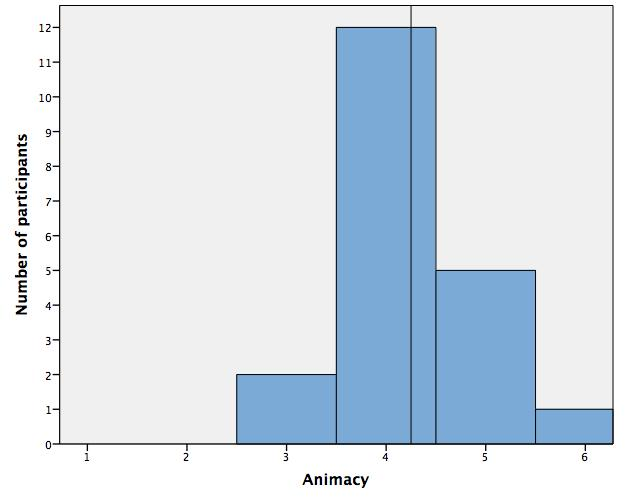
\includegraphics[width=\textwidth]{AnimacyBaseline.jpeg}
		\caption{Animacy histogram in the control condition.}
		\label{fig:animacy_baseline}
	\end{minipage}
	\hspace{2mm}
	\begin{minipage}[b]{.2\textwidth}
		\centering
		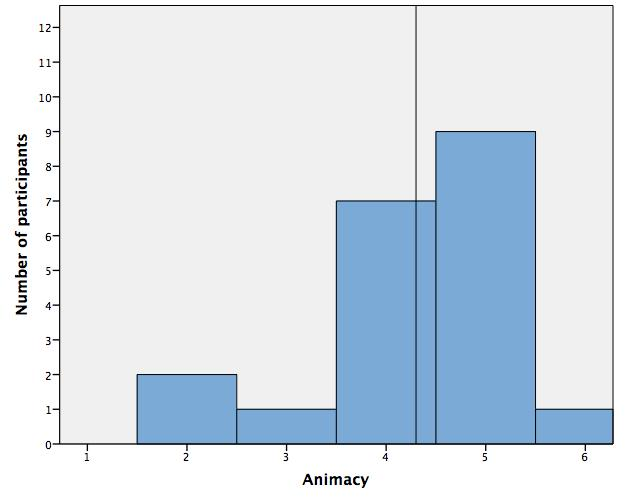
\includegraphics[width=\textwidth]{AnimacyRapport.jpeg}
		\caption{Animacy histogram in the rapport condition.}
		\label{fig:animacy_rapport}
	\end{minipage}
\end{figure}

\textbf{Answer}: There is no definite proof that the current system improves the agent's liveness.

\subsection*{\textbf{\textit{Do rapport strategies affect the perceived intelligence?}}}

Similar to likeability and animacy, the perceived intelligence distributions on  conditions C and R are not normal ($sig_C=0$ and $sig_R=0.002$), therefore we compare both conditions with the \textit{Mann–Whitney U} statistical test. The histogram's shapes (Figures~\ref{fig:intelligence_baseline} and~\ref{fig:intelligence_rapport}) are dissimilar ($sig=1.0$), therefore we only compare the mean scores: 5.1±0.553 and 5.0±0.918, on conditions C and R, respectively.

\begin{figure}[H]
	\centering
	\begin{minipage}[b]{.2\textwidth}
		\centering
		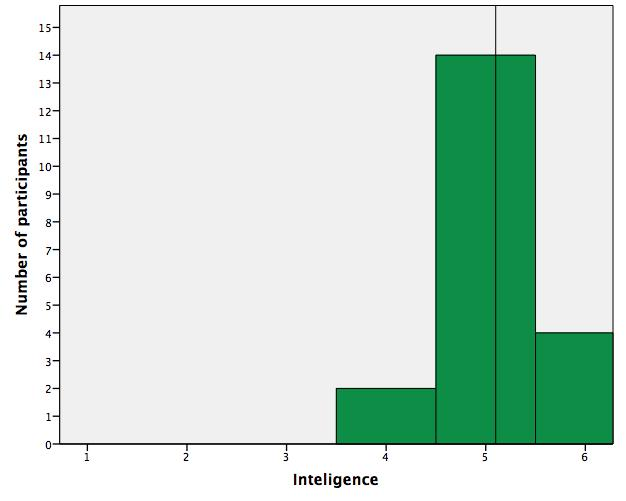
\includegraphics[width=\textwidth]{PerceivedIntelligenceBaseline.jpeg}
		\caption{Perceived intelligence histogram in the control condition.}
		\label{fig:intelligence_baseline}
	\end{minipage}
	\hspace{2mm}
	\begin{minipage}[b]{.2\textwidth}
		\centering
		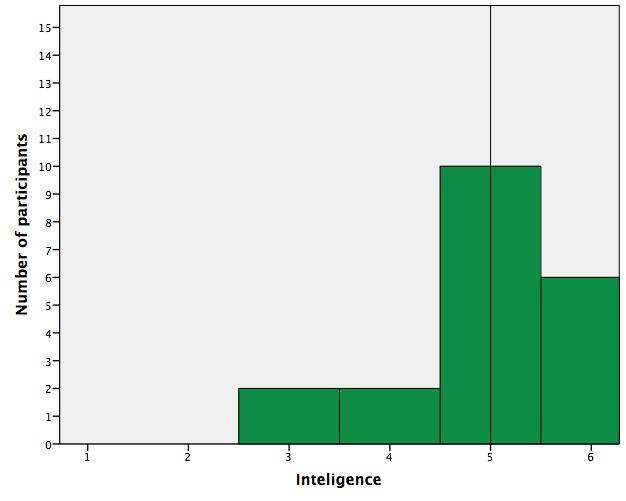
\includegraphics[width=\textwidth]{PerceivedIntelligenceRapport.jpeg}
		\caption{Perceived intelligence histogram in the rapport condition.}
		\label{fig:intelligence_rapport}
	\end{minipage}
\end{figure}


\textbf{Answer}: There is no statistical proof that the rapport strategies have an effect on the agent's perceived intelligence.
 
\subsection*{\textit{\textbf{Are the rapport strategies effective in establishing closer relationships between humans and agents?}}}

In order to answer the last hypothesis, we compare the proximities answers between conditions C (Figure~\ref{fig:proximity_baseline}) and R (Figure~\ref{fig:proximity_rapport}) using a 7-item scale question. In both conditions, proximity follows a normal distributions ($sig_C=0.203$ and $sig_R=0.304$), therefore we use the independent \textit{t-test} statistic test which yielded the statistical significance value of 0.694 ($>0.05$), consequently we reject the null hypothesis.

\begin{figure}[ht]
	\centering
	\hspace{5mm}
	\begin{minipage}[b]{.2\textwidth}
		\centering
		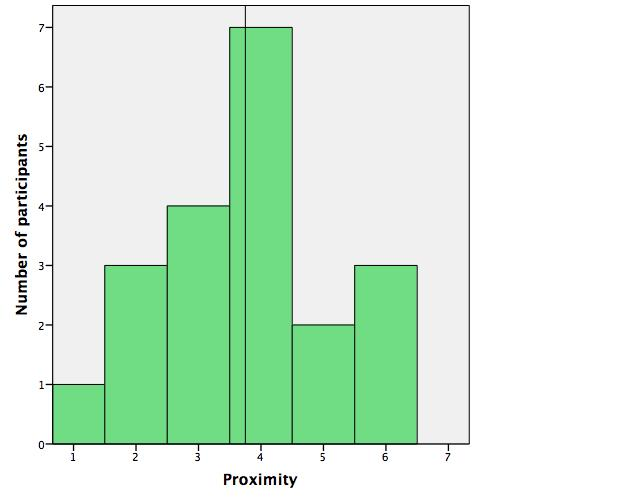
\includegraphics[width=\textwidth]{EmysBaseline.jpeg}
		\caption{Proximity histogram in the control condition.}
		\label{fig:proximity_baseline}
	\end{minipage}
	\hspace{2mm}
	\begin{minipage}[b]{.2\textwidth}
		\centering
		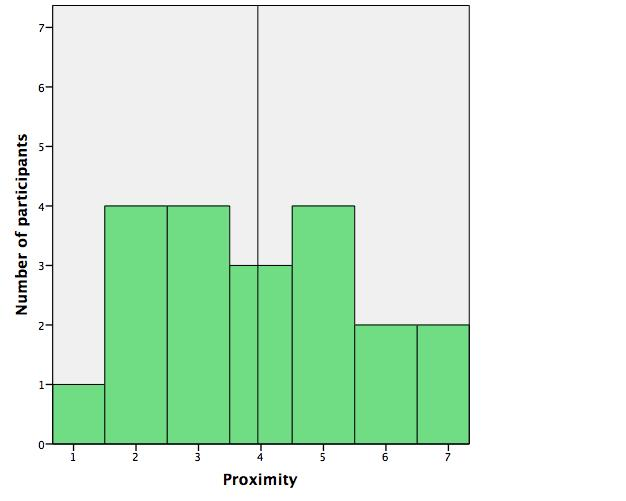
\includegraphics[width=\textwidth]{EmysRapport.jpeg}
		\caption{Proximity histogram in the rapport condition.}
		\label{fig:proximity_rapport}
	\end{minipage}
\end{figure}


\textbf{Answer}: Despite the small increase of 0.2 on the mean score from condition C to R, the impact of the rapport strategies on proximity are inconclusive.